\section{Modelo de interfaces}
En esta secci\'on se describen las pantallas que componen el sistema,
mostrando los campos que componen los formularios, as\'i como los mensjaes
de ayuda o error que puedan presentarse a lo largo de la ejecuci\'on.

\subsection{Ingreso al sistema}

\begin{figure}[h]
  \centering
    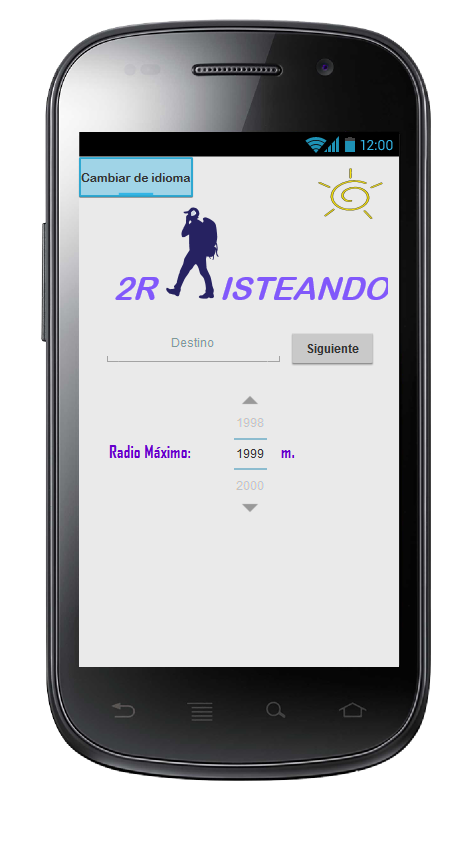
\includegraphics[width=5cm,height=8cm]{Imagenes/VistasSistema/VistaPrincipal.png}
  \caption{Vista principal del sistema.}  
\end{figure}

\newpage
\subsection{Despliegue de informaci\'on}
\begin{figure}[h]
  \centering
    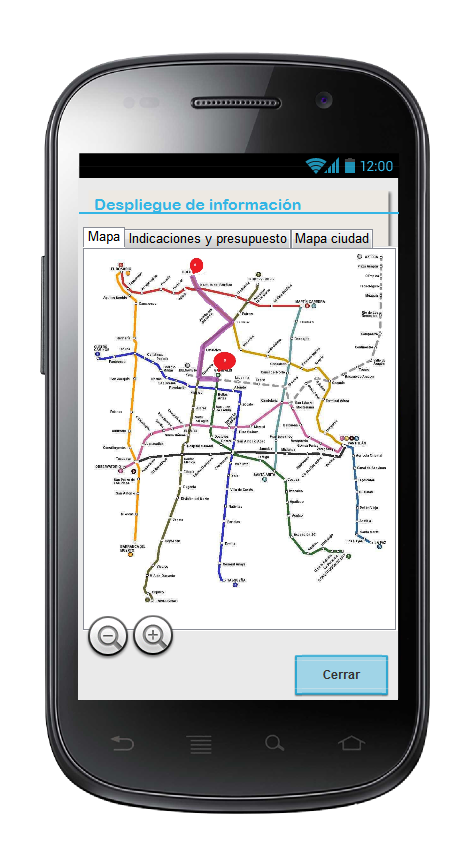
\includegraphics[width=5cm,height=8cm]{Imagenes/VistasSistema/CU1_1.png}
  \caption{VCU1.1 Vista para ver la ruta en el medio de transporte.}  
\end{figure}

\begin{figure}[h]
  \centering
    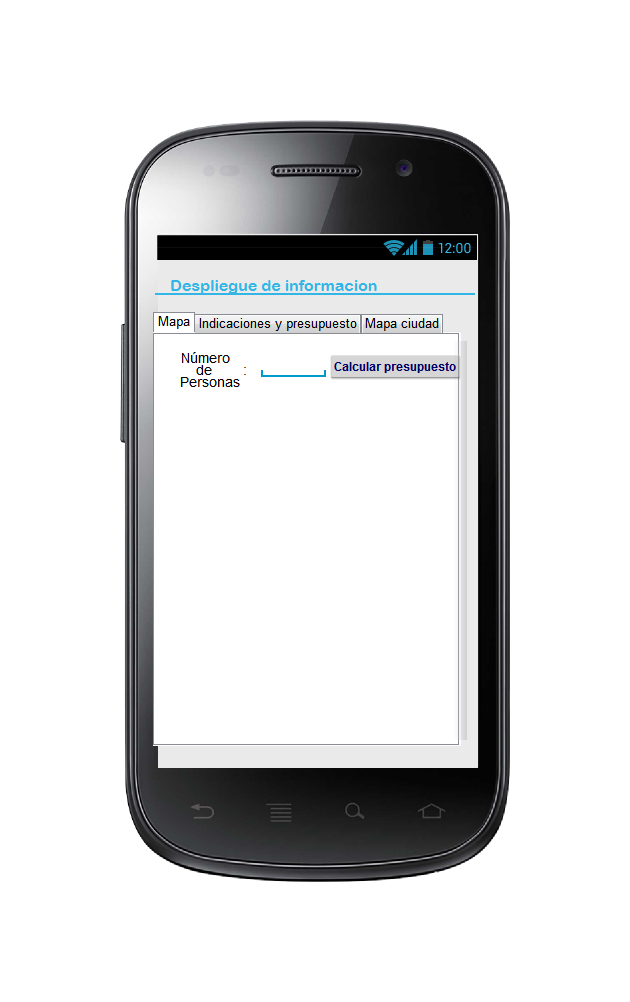
\includegraphics[width=5cm,height=8cm]{Imagenes/VistasSistema/CU1_2.png}
  \caption{VCU1.2 Vista para ver informaci\'on del viaje}  
\end{figure}

\begin{figure}[h]
  \centering
    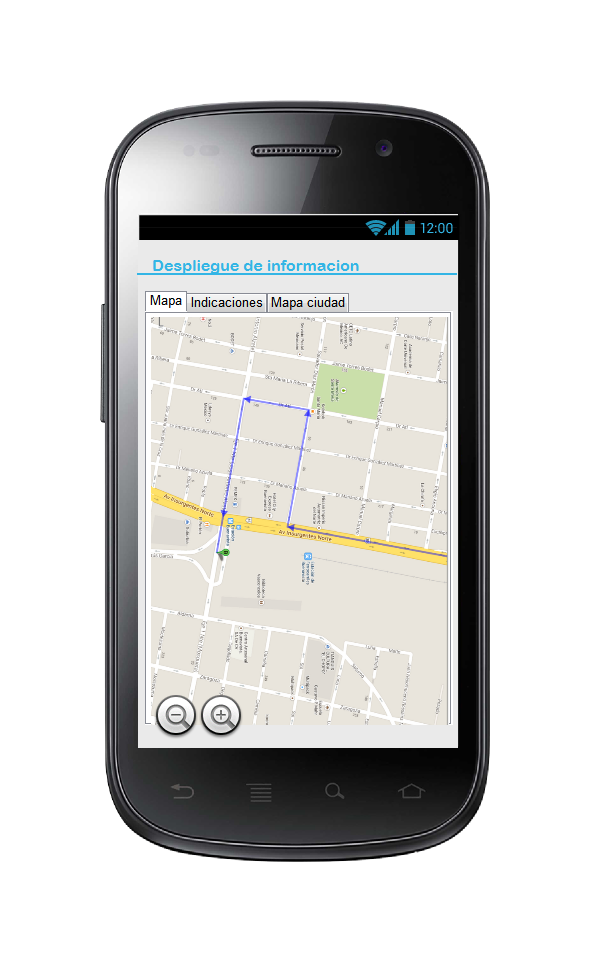
\includegraphics[width=5cm,height=8cm]{Imagenes/VistasSistema/CU1_3.png}
  \caption{VCU1.3 Vista para ver el mapa de la ciudad}  
\end{figure}

\newpage
\subsection{Administrar el itinerario}

\begin{figure}[h]
  \centering
    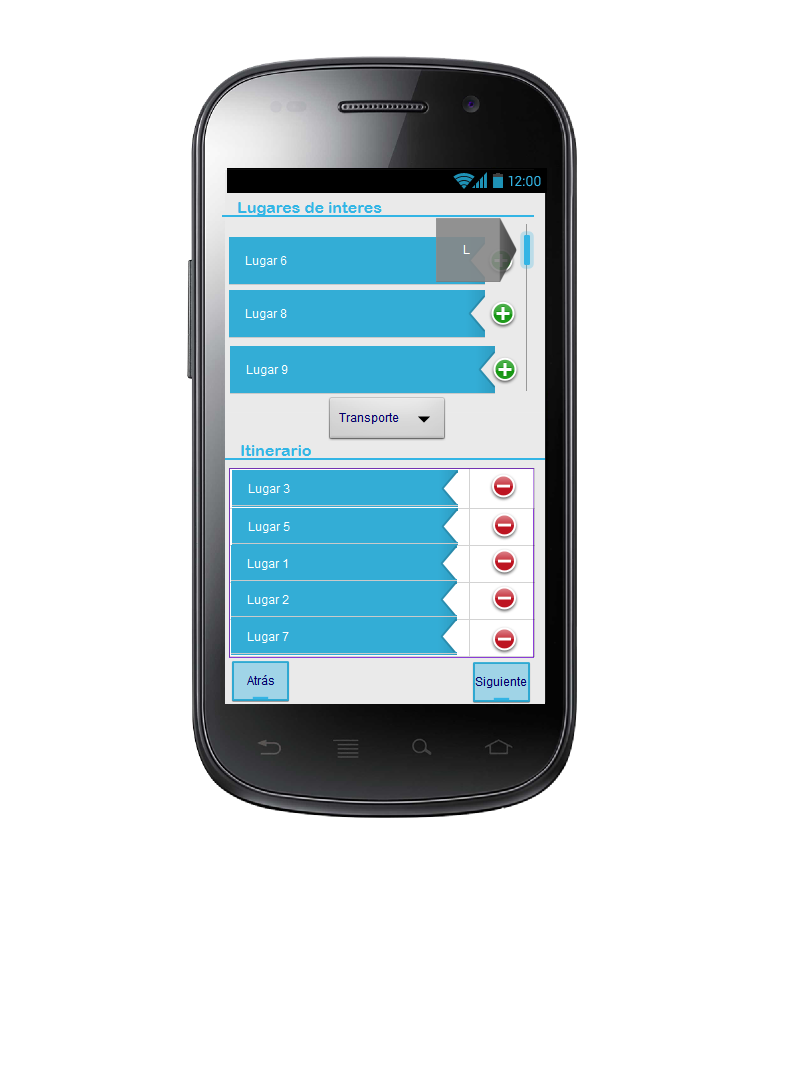
\includegraphics[width=5cm,height=8cm]{Imagenes/VistasSistema/CU2.png}
  \caption{VCU2 Vista para administrar el itinerario.}  
\end{figure}

\newpage
\subsection{Agregar un lugar}

\begin{figure}[h]
  \centering
    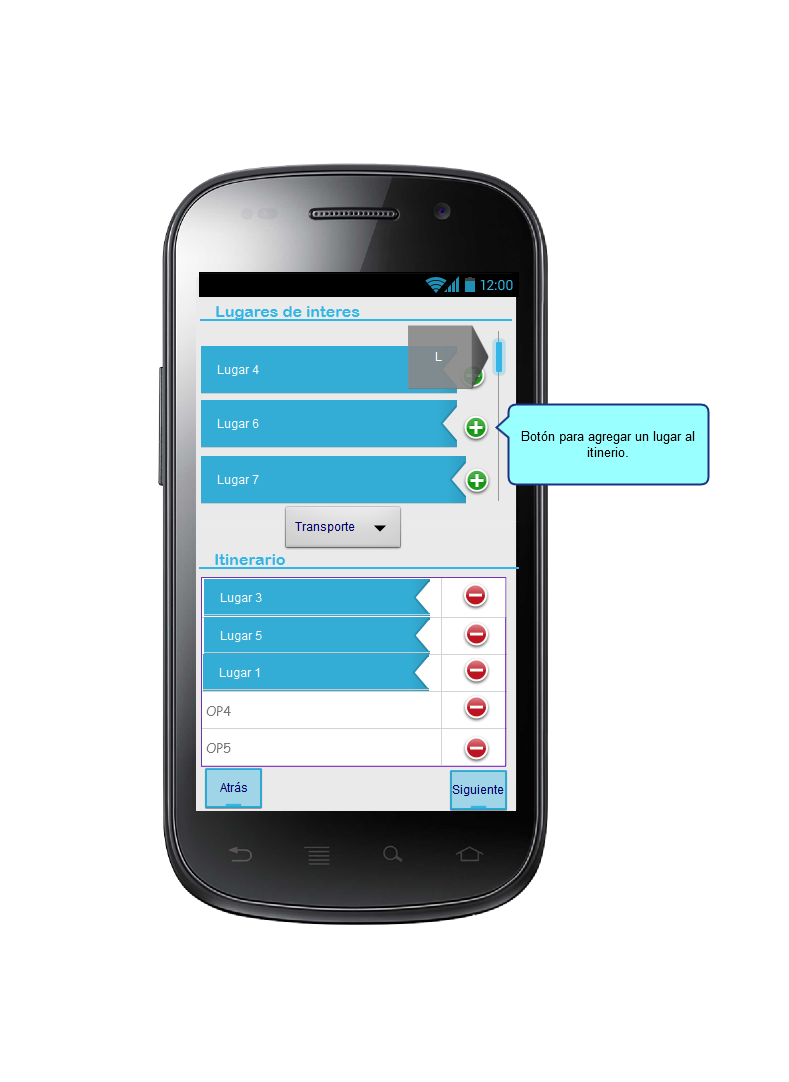
\includegraphics[width=5cm,height=8cm]{Imagenes/VistasSistema/CU2_1.png}
  \caption{VCU2.1 Vista para agregar un lugar al itinerario.}  
\end{figure}

\newpage
\subsection{Eliminar un lugar}

\begin{figure}[h]
  \centering
    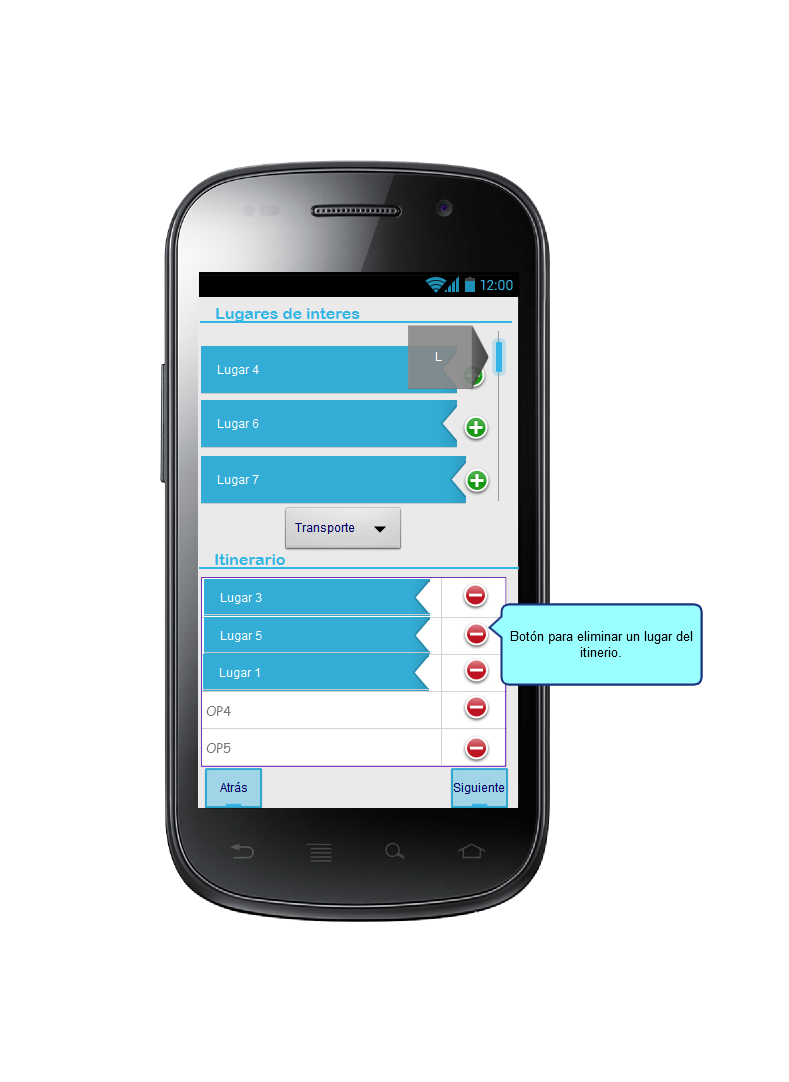
\includegraphics[width=5cm,height=8cm]{Imagenes/VistasSistema/CU2_2.png}
  \caption{VCU2.1 Vista para eliminar un lugar al itinerario.}  
\end{figure}

\newpage
\subsection{Cambiar idioma}

\begin{figure}[h]
  \centering
    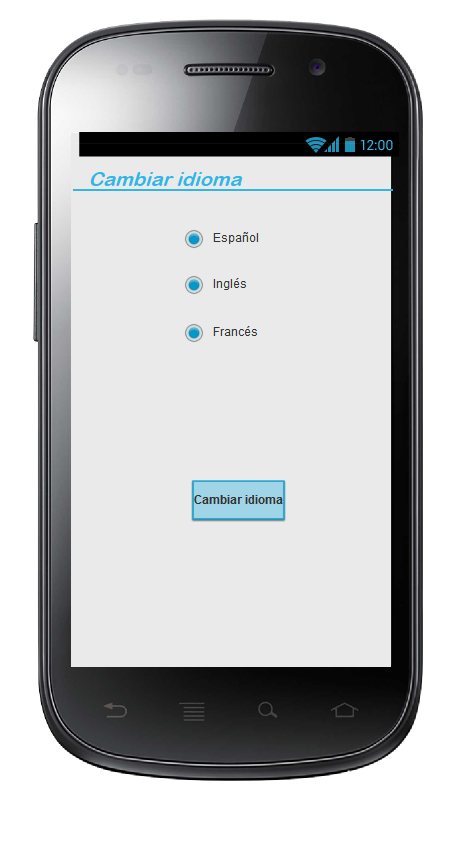
\includegraphics[width=5cm,height=8cm]{Imagenes/VistasSistema/CU3.png}
  \caption{VCU3 Vista para cambiar el idioma del sistema.}  
\end{figure}

  